\documentclass{article}

\usepackage{arxiv}

\usepackage[utf8]{inputenc} % allow utf-8 input
% \usepackage[T1]{fontenc}    % use 8-bit T1 fonts
\usepackage[T1,T2A]{fontenc}      % keep Latin fonts (T1) and add Cyrillic (T2A)
\usepackage[russian,english]{babel}
\usepackage{hyperref}       % hyperlinks
\usepackage{url}            % simple URL typesetting
\usepackage{booktabs}       % professional-quality tables
\usepackage{amsfonts}       % blackboard math symbols
\usepackage{amsmath}        % math
\usepackage{nicefrac}       % compact symbols for 1/2, etc.
\usepackage{microtype}      % microtypography
\usepackage{lipsum}		% Can be removed after putting your text content
\usepackage{graphicx}
\usepackage[table]{xcolor} %color tables
\usepackage{doi}
% \usepackage{natbib}
\usepackage[sort&compress]{natbib}
\setcitestyle{numbers}
\citestyle{nature}
\bibliographystyle{unsrtnat}

\begin{titlepage}
% \newpage

\begin{center}
NATIONAL RESEARCH UNIVERSITY\\
HIGHER SCHOOL OF ECONOMICS
\\
\bigskip
Faculty of Computer Science\\
Bachelor’s Programme “Data Science and Business Analytics”
\end{center}


\vspace{7em}

\begin{center}
{\bf BACHELOR'S THESIS}\\
%Выберите какой у вас проект
{\bf Research Project on the Topic:}\\
%{\bf Software Project on the Topic:}\\
{\bf Methods of Evaluation of Diffusion Model Hallucinations}\\
\end{center}

\vspace{2em}

{\bf Submitted by the Student: \vspace{2mm}}

\begin{tabular}{l@{\hskip 1.5cm}l}
group \#\foreignlanguage{russian}{БПАД}213, 4th year of study & 
Pakhurov Fedor Konstantinovich
\end{tabular}

% Обычно у вас есть один научный руководитель, и это человек, с которым вы работаете над проектом. Иногда по формальным причинам у вас будет руководитель (штатный сотрудник Вышки) и соруководитель (тот, с кем вы работаете), — об этом вам сообщит учебный офис (в случае с ВКР) или ЦППРиП (в случае с курсовым проектом). Также, если кто-то дополнительно вам помогал, то его можно указать как консультанта. 

%ваш официальный научник (из ВШЭ)
\vspace{1em}
{\bf Approved by the Supervisor: \vspace{2mm}}

\begin{tabular}{l@{\hskip 1.5cm}l}
Lukianchenko Petr Pavlovich, \\
Senior Lecturer, \\
Big Data and Information Retrieval School \\ 
\end{tabular}

% со-руководитель (если есть)
%\vspace{1em}
%{\bf Co-supervisor: \vspace{2mm}}

%{\setstretch{1.1}
%\begin{tabular}{l@{\hskip 1.5cm}l}
%Petrova Ekaterina Maksimovna\\
%Research Fellow\\
%AO "Neural networks in the wild" 
%\end{tabular}}

% консультант (если есть)
%\vspace{1em}
%{\bf Consultant: \vspace{2mm}}

%{\setstretch{1.1}
%\begin{tabular}{l@{\hskip 1.5cm}l}
%Ivanova Ekaterina Maksimovna\\
%Research Fellow\\
%AO "Neural networks in the wild" 
%\end{tabular}}

\mbox{}
  \\
  \\
  \\
  \\
  \\
  \\
  \\
  \\
  \\
  \\
  \\
  \\
  \\
  \\
  \\
  \\
  \\
  \\
  \\
  \\
  \\
  \\
  \\
  \\
  \\
  \\
  \\
  \\
  \\
\mbox{}

% \vspace*{\fill}

\begin{center}
Moscow 2025
\end{center}

\end{titlepage}

\title{Methods of Evaluation of Diffusion Model Hallucinations}

%\date{September 9, 1985}	% Here you can change the date presented in the paper title
%\date{} 					% Or removing it

% \author[Fedor K. Pakhurov]{DSBA213, HSE University, Moscow, Russia}
\author{
    Fedor K. Pakhurov\\
    DSBA213,\\
    HSE University,\\
    Moscow, Russia\\
    \texttt{fpakhurov@gmail.com}
}

% Uncomment to remove the date
\date{}

% Uncomment to override  the `A preprint' in the header
\renewcommand{\headeright}{Bachelor's Thesis}
\renewcommand{\undertitle}{Bachelor's Thesis}
\renewcommand{\shorttitle}{Methods of Evaluation of Diffusion Model Hallucinations}

%%% Add PDF metadata to help others organize their library
%%% Once the PDF is generated, you can check the metadata with
%%% $ pdfinfo template.pdf
\hypersetup{
pdftitle={Methods of Evaluation of Diffusion Model Hallucinations},
pdfsubject={q-bio.NC, q-bio.QM},
pdfauthor={Fedor K. Pakhurov},
pdfkeywords={Diffusion models, Hallucination detection, Complexity–entropy analysis},
}

\begin{document}
\maketitle

\begin{abstract}
Diffusion models excel at image synthesis yet still emit hallucinations. Motivated by recent calls for rigorous evaluation, we present a model‑agnostic pipeline that detects and ranks hallucinations using Rényi complexity–entropy curves and unsupervised clustering. The procedure embeds each signal in the two‑dimensional complexity–entropy plane, then partitions the resulting cloud with KMeans to flag outliers. We construct a benchmark of real, periodic, stochastic and noise sequences and show that the learned cluster envelope transfers to local traces of diffusion‑model images, providing a lightweight hallucination‑likelihood oracle for future safety studies.
\end{abstract}

\vspace{1.5\baselineskip} 

% \begin{abstractru}
%     Диффузионные модели впечатляют качеством изображений, но всё ещё порождают галлюцинации. Отвечая на запросы строгой оценки, мы предлагаем архитектурно‑независимый конвейер, обнаруживающий и ранжирующий галлюцинации с помощью кривых сложности‑энтропии Реньи и неконтролируемой кластеризации. Сигналы отображаются в двумерную плоскость «сложность–энтропия», после чего облако точек разделяется алгоритмами KMeans, иерархической кластеризацией Уорда и DBSCAN для выявления выбросов. Публикуется эталонный набор реальных, периодических, стохастических и шумовых последовательностей; показано, что полученная граница кластеров переносится на локальные срезы изображений, превращая CE + DBSCAN в лёгкий оракул вероятности галлюцинаций для исследований безопасности.
% \end{abstractru}


\keywords{Diffusion models \and Hallucination evaluation \and Complexity–entropy analysis}

\clearpage
\tableofcontents


% ------------------------------------------------------------------
\clearpage
\section{Aim and Objectives}\label{sec:aim}

\textbf{Aim.}\;
Develop a rigorous method for detecting, classifying, and
quantitatively evaluating hallucinations in the outputs of
diffusion‑based generative models.

\medskip
\noindent\textbf{Objectives.}
\begin{enumerate}
\item \textbf{Literature survey:} Review current hallucination‑detection
      techniques for diffusion and related generative architectures,
      analysing underlying assumptions and limitations.
\item \textbf{Method design and implementation:} Propose and implement an
      algorithm that integrates complexity–entropy measures and
      clustering strategies into the diffusion pipeline.
\item \textbf{Empirical evaluation:} Benchmark the proposed method
      against established baselines, report quantitative metrics, and
      analyse robustness across datasets and model configurations.
\end{enumerate}

% ------------------------------------------------------------------
\section{Problem Statement}\label{sec:problem}

Diffusion models achieve state‑of‑the‑art fidelity in image and signal
generation, yet they frequently emit hallucinations — outputs that
depart from real‑world semantics or statistics.  Existing evaluation
protocols mainly quantify distributional divergence from training
data, providing limited insight into hallucinations that arise in
novel generations.  Consequently, practitioners lack reliable tools
to flag hallucinated content and to measure hallucination severity.
This work addresses the gap by devising a principled detection and
evaluation framework that operates on unseen data and yields
actionable metrics.

% ------------------------------------------------------------------
\section{Relevance of the Topic}\label{sec:relevance}

Diffusion models underpin creative design, scientific visualisation,
and decision‑support systems; undetected hallucinations erode user
trust and propagate misinformation.  Industry calls for lightweight
quality‑assurance pipelines, while academia seeks deeper understanding
of generative reliability.  A methodology that accurately detects and
evaluates hallucinations therefore holds immediate significance: it
safeguards practical applications, guides model development toward
verifiable performance, and advances the broader agenda of aligning
generative AI with real‑world requirements.

% ------------------------------------------------------------------
\section{Review of Existing Approaches}\label{sec:related}

\subsection{Latent Mode‑Interpolation Analysis}
Mode‑interpolation tracks the variance of reverse‑diffusion
trajectories to detect out‑of‑support generations
\citep{NEURIPS2024_f29369d1}.% :contentReference[oaicite:0]{index=0}
The variance over the last $K$ steps is
\begin{equation}
\sigma^{2}= \frac{1}{K}\sum_{k=1}^{K}\bigl\lVert
x_{t_k}-\bar{x}\bigr\rVert_2^{2}, \qquad
\bar{x}=\frac{1}{K}\sum_{k=1}^{K}x_{t_k}.
\label{eq:traj_var}
\end{equation}
The limitations are: the thresholds are model‑specific, the metric is
global, and full‑trajectory storage increases cost.

\subsection{Scene‑Graph Question–Answering Evaluation}
Qin \emph{et al.} convert a generated image into a scene graph and
query a language model; answer–prompt mismatches reveal hallucinations
\cite{qin2024evaluatinghallucinationtexttoimagediffusion}.
Performance is bounded by vision and relation‑extraction accuracy, and
run‑time is dominated by LLM inference.

\subsection{Local Diffusion Decomposition}
Kim~\emph{et al.} mitigate structural hallucination via local
out-of-distribution‑aware diffusion and fusion \citep{10.1007/978-3-031-73004-7_6}.% :contentReference[oaicite:2]{index=2}
However, OOD mask quality and multiple sampling passes limit
practicality.

\subsection{Complexity–Entropy Analysis}\label{sec:ce}

\paragraph{Permutation entropy.}
For a scalar series $X=(x_1,\dots,x_N)$, embedding dimension $d$,
delay~$\tau$, and permutation frequencies $P=\{p_i\}$,
\begin{equation}
H_S(d,\tau)=-\sum_{i=1}^{d!}p_i\log p_i, \quad
h_S=\frac{H_S}{\log d!}\in[0,1].
\label{eq:perm_entropy}
\end{equation}

\paragraph{Jensen–Shannon complexity.}
With the uniform distribution $P_u$ and $m_i=\tfrac12(p_i+1/d!)$,
\begin{align}
D_{\mathrm{JS}}(P,P_u) &=
\tfrac12\sum_{i}\Bigl[p_i\log\frac{p_i}{m_i}+
\frac{1}{d!}\log\frac{1/d!}{m_i}\Bigr],\\[2pt]
C_{\mathrm{JS}} &=
\frac{D_{\mathrm{JS}}(P,P_u)}{D_{\mathrm{JS}}^{\max}}\;h_S.
\end{align}
Plotting $(h_S,C_{\mathrm{JS}})$ yields the complexity–entropy
causality plane (CECP) \citep{PhysRevE.95.062106}.% :contentReference[oaicite:3]{index=3}

\paragraph{Rényi complexity–entropy curve.}
Replacing Shannon by Rényi entropy produces curves that discriminate
chaotic, stochastic, and periodic signals
\citep{RePEc:eee:phsmap:v:498:y:2018:i:c:p:74-85}.% :contentReference[oaicite:4]{index=4}

\paragraph{Proposed Detection pipeline.}
\begin{enumerate}
\item Convert each image (or latent) to a 1‑D signal.
\item Compute permutation frequencies $P$ for fixed $(d,\tau)$.
\item Evaluate $(h,C)$ and embed in CECP or Rényi curve space.
\item Cluster via DBSCAN; clusters outside the validated envelope are
      labelled hallucinations.
\end{enumerate}

Difficulties include sensitivity to $(d,\tau)$, factorial growth of
$d!$, and noise‑inflated entropy
\citep{2016NTA.....7...21C}.% :contentReference[oaicite:5]{index=5}

\subsection{Comparative Limitations}
\begin{itemize}
\item \emph{Coverage:} global (Mode‑Interpolation), prompt‑conditional
      (SG‑QA), structural (Local Diffusion), distributional (CE).
\item \emph{Ground‑truth needs:} only SG‑QA requires prompt annotations.
\item \emph{Computation:} Local Diffusion and SG‑QA are costly; CE is
      lightweight but sensitive to hyper‑parameters.
\end{itemize}

\subsection{Conclusion and Outlook}\label{sec:conclusion}

No single method currently addresses all hallucination modes.  A
hybrid framework that fuses local structural cues with global
complexity–entropy descriptors promises broader coverage and more
consistent evaluation.  Future work will integrate the proposed CE‑based
detector into diffusion pipelines, expand evaluation datasets, and
perform parameter studies across entropy‑complexity variants.

% ------------------------------------------------------------------
\section{Method Selection and Justification}\label{sec:method_choice}

\subsection{Complexity–Entropy (CE) Feature Space}

\begin{enumerate}
\item \textbf{Model‑agnostic representation.}
      CE descriptors operate directly on the statistical ordering of
      samples; they do not depend on internal model states and are
      therefore applicable to any generative architecture encountered
      later in the project.
\item \textbf{Sensitivity to irregular structure.}
      The combination of normalised permutation entropy $h_S$
      (Eq.~\ref{eq:perm_entropy}) and statistical complexity
      $C_{\mathrm{JS}}$ distinguishes stochastic, periodic, and chaotic
      regimes.  Hallucinations — being atypical mixtures of such regimes — 
      are expected to form outlying manifolds in the CE plane.
\item \textbf{Computational efficiency.}
      CE metrics require only ordinal‑pattern counting; the complexity
      scales linearly with signal length and is amenable to fast vectorised
      implementations, enabling large‑scale screening.
\item \textbf{Interpretability.}
      The CE causality plane provides a two‑dimensional visual summary
      in which regions associated with plausible data can be empirically
      bounded, offering an intuitive decision surface for downstream
      users.
\end{enumerate}

\subsection{Clustering Strategy}

\vspace{-0.3\baselineskip}
\paragraph{Clustering (supposedly DBSCAN/HDBSCAN).}
\begin{itemize}
\item \emph{Non‑parametric.}  No prior on the number of clusters is
      required, matching the unsupervised nature of hallucination
      discovery.
\item \emph{Adaptive to irregular shapes.}  Hallucination manifolds may be
      sparse or elongated in CE space; density‑based methods should capture
      such structures better than $k$‑means or Gaussian mixtures; to be tested.
\item \emph{Outlier labelling.}  Points with low neighbourhood density
      are automatically marked as noise, providing a principled
      hallucination flag without additional thresholds.
\end{itemize}

\vspace{-0.6\baselineskip}
\paragraph{Alternative considered and rejected.}
Spectral and hierarchical clustering were evaluated but found either
computationally heavier (spectral) or less stable under parameter
perturbations (linkage methods) when applied to CE embeddings of
high‑resolution imagery.

% ──────────────────────────────────────────────────────────────────
\section{Work Plan}\label{sec:work_plan}

\bigskip
\textbf{Phase I – Time-Series Clustering Module}
\begin{enumerate}
\item Data preparation (canonical constant/periodic/stochastic/noise/real series).
\item Feature-engineering module (permutation entropy, Rényi CE curves).
\item Clustering and decision layer (DBSCAN / KMeans / analogous).
\item Validation and robustness analysis (silhouette, purity, etc.).
\end{enumerate}

\textbf{Phase II – Image-Based Extension}
\begin{enumerate}
\item Gather three balanced subsets: \emph{Real images}, \emph{Error–less
      diffusion}, \emph{Diffusion with errors}.
\item Formulate a discriminative metric
      (Eq.~\ref{eq:hall_score}, below) and a tunable convolutional
      feature extractor.
\item Grid-search the convolutional hyper-parameters jointly with the
      CE-clustering model.
\item Integrate the image module with the time-series detector and
      evaluate cross-domain generalisation.
\end{enumerate}
% ------------------------------------------------------------------
\section{Time-Series Clustering}\label{sec:results}

\subsection{Mathematical Model}

For every time–series sample \(X=\{x_t\}_{t=1}^{N}\) we first embed the
signal in the ordinal pattern space of order \(d=5\) and delay
\(\tau=1\).  Let \(P=\{p_i\}_{i=1}^{d!}\) be the corresponding
permutation‐probability vector.  For a selected set of Rényi parameters
\(\alpha \in \mathcal{A} = \{0.0,0.1,\dots,1.0\}\) we compute

\begin{align}
H_\alpha(P)
  &=\frac{1}{1-\alpha}\log\!\Bigl[\sum_{i=1}^{d!} p_i^{\,\alpha}\Bigr],\\
C_\alpha(P)
  &=\Bigl[\frac{D_{\mathrm{JS},\alpha}(P,P_u)}%
                 {D^{\max}_{\mathrm{JS},\alpha}}\Bigr]\;
     \frac{H_\alpha(P)}{H^{\max}_\alpha},
\end{align}

yielding a \(2|\mathcal{A}|\)-dimensional feature vector  
\(\mathbf{f}(X)=[H_\alpha,C_\alpha]_{\alpha\in\mathcal{A}}\).

\subsection{Experimental Data}

Five canonical classes were synthesised or collected:

\begin{itemize}
\item \textbf{Real}: WTI crude spot‑price daily series (2020–2025)~\citep{EIA_WTI_DCOILWTICO};
\item \textbf{Noise}: standard Gaussian white noise;
\item \textbf{Stochastic}: fractional Brownian motion (\(H\!=\!0.7\));
\item \textbf{Constant}: DC signal with \(1\%\) jitter;
\item \textbf{Periodic}: sinusoid with additive \(N(0,0.02)\) noise.
\end{itemize}

Each class contributes \(10\) sequences of length \(2^{12}\),
resulting in \(N=50\) samples.

\subsection{Experimental Setup}\label{sec:setup}

For each time‑series example we fix permutation order \(d_x = 5\) and
delay \(\tau = 1\).  We then sweep the Rényi parameter over the grid
\(\alpha \in \mathcal{A} = \{0.0,0.1,\dots,1.0\}\) (\(|\mathcal{A}|=10\)).
Every \emph{single} \(\alpha\) produces one point
\((H_\alpha,\,C_\alpha)\) in the two‑dimensional complexity–entropy
plane; taken together, the 10 points trace a short \emph{CE curve}.  In
our clustering study we simply treat the union of all points from all
curves as the data cloud to be partitioned.\footnote{Because the CE
plane is already two‑dimensional, no further vector concatenation is
required; the silhouette scores therefore refer to the direct
\((H,C)\)-scatter, not to any higher‑dimensional embedding.}

% ──────────────────────────────────────────────────────────────────
\subsection{Parameter-Sensitivity Study (clustering hyper-parameters)}
\label{sec:grid}
% ──────────────────────────────────────────────────────────────────

The analysis is completed by a
\emph{clustering-level} grid search.  Three independent grids were
examined:

\begin{itemize}
\item \textbf{KMeans:}\;$k\in\{4,5,6,7\}$,\; $n_{\textit{init}}=10$;
\item \textbf{Agglomerative (Ward):}\;$k\in\{4,5,6,7\}$;
\item \textbf{DBSCAN:}\;$\varepsilon\in\{0.015,0.020,0.025\}$,\;
      $\textit{min\_samples}\in\{2,3\}$.
\end{itemize}

The CE point cloud described in \S\ref{sec:setup} was re-clustered
under every combination.  Table~\ref{tab:grid_silhouette} shows the
\emph{best} silhouette score achieved by each algorithm. 

KMeans with $k=5$ achieves the highest silhouette (0.72) while keeping the
decision surface simple and reproducible; it is therefore selected as the
default clusterer in both Phase I and Phase II.

\begin{table}[h!]
\centering
\begin{tabular}{@{}lccc@{}}
\toprule
Algorithm & Best hyper-parameters & Silhouette score & Rank \\
\midrule
KMeans                    & $k=5$                       & \textbf{0.720} & 1 \\
Agglomerative (Ward)      & $k=5$                       & 0.706          & 2 \\
DBSCAN                    & $\varepsilon=0.020,\;m\!=\!2$ & 0.364          & 3 \\
\bottomrule
\end{tabular}
\caption{Best silhouette scores over the clustering hyper-parameter
grid.}
\label{tab:grid_silhouette}
\end{table}


\begin{figure}[h!]
\centering
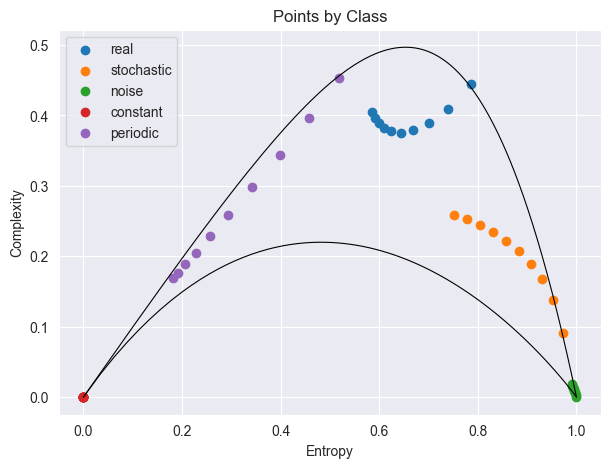
\includegraphics[width=.7\linewidth]{orig_classes.png}
\caption{Ground‑truth classes in the \((H_{1},C_{1})\) plane
(\emph{real}, \emph{noise}, \emph{stochastic}, \emph{constant},
\emph{periodic}).}
\label{fig:orig_classes}
\end{figure}

\begin{figure}[h!]
\centering
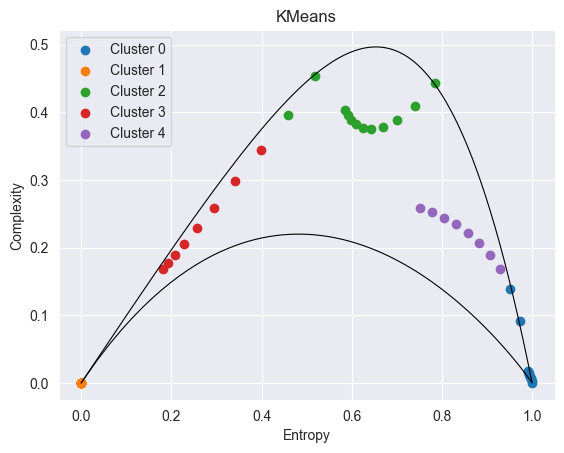
\includegraphics[width=.7\linewidth]{kmeans_ce_plane.png}
\caption{KMeans clusters (\(k=5\)).}
\label{fig:kmeans}
\end{figure}

\begin{figure}[h!]
\centering
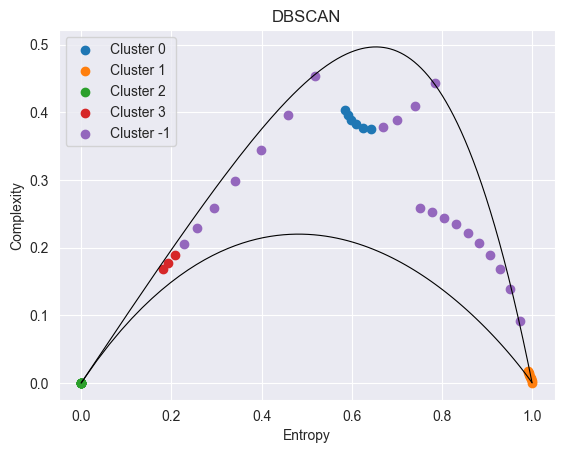
\includegraphics[width=.7\linewidth]{dbscan_ce_plane.png}
\caption{DBSCAN clusters (\(\varepsilon=0.02\)).}
\label{fig:dbscan}
\end{figure}

\begin{figure}[h!]
\centering
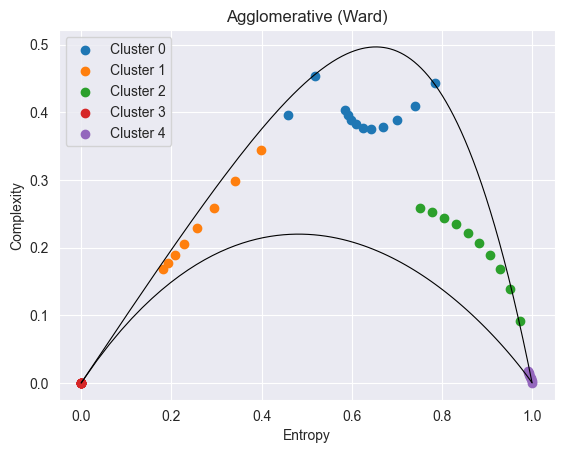
\includegraphics[width=.7\linewidth]{agglo_ce_plane.png}
\caption{Agglomerative‑Ward clusters (\(k=5\)).}
\label{fig:agglo}
\end{figure}

% ──────────────────────────────────────────────────────────────────
\section{Image-Based Hallucination Evaluation}
\label{sec:image_module}

\subsection{Dataset collection}
We have collected a balanced corpus of 100 images, drawing approximately 32 items for each of three mutually–exclusive classes: \emph{Real} photographs, \emph{Good} diffusion outputs, and \emph{Bad} (hallucinated or failed) diffusion outputs.\citep{Lin2014COCO,MidjourneyWebsite}
The \emph{Real} subset was randomly sampled from the MS~COCO~\citep{Lin2014COCO} and FFHQ~\citep{Karras2019FFHQ} datasets.
High-quality \emph{Good} generations were taken from crowd-curated showcases of Midjourney~\citep{MidjourneyWebsite}, the community DALL\textperiodcentered E~3 gallery~\citep{DALLE3Gallery}, the Stable Diffusion XL reference samples~\citep{Podell2023SDXL}, Google’s Imagen~\citep{Saharia2022Imagen}, and Mage~\citep{MageSpace} and Lexica~\citep{LexicaArt} diffusion models' galleries.
Hallucination or failure examples constituting the \emph{Bad} class were collected from Everypixel’s taxonomy of AI hallucinations~\citep{EverypixelHalluc}, the r/StableDiffusion ``failures'' thread~\citep{RedditStableFail}, and the Bored Panda ``AI Art Fails'' article~\citep{BoredPandaFails}.

\subsection{Metric for Hyper-parameter Selection}
For any candidate parameter set \(\Theta\) the quality of the detector
is measured by
\begin{equation}
\label{eq:hall_score}
\text{score}(\Theta)=
\underbrace{\mathbb{E}\!\bigl[p_{\mathrm{hall}}\mid{\text{bad}},
\Theta\bigr]}_{\text{want \emph{high}}}
-
\underbrace{\mathbb{E}\!\bigl[p_{\mathrm{hall}}\mid
{\text{real, good}},\Theta\bigr]}_{\text{want \emph{low}}},
\end{equation}
where \(p_{\mathrm{hall}}\) is the \emph{total probability mass} of all
clusters flagged as hallucination-like.  A
large positive score indicates that \(\Theta\) pushes \emph{bad} images
into the ``Noise/Stochastic'' region while keeping \emph{real} and
\emph{good} images outside.

\subsection{Search Space and Tuned Parameters}
The convolutional front-end is characterised by  
\(\texttt{kernel\_size}\in\{3,5\}\),  
\(\texttt{stride}\in\{1,2\}\),  
\(\texttt{padding}\in\{0,1\}\),  
\(\texttt{out\_channels}\in\{1,2,4\}\),
resulting in \(2\times2\times2\times3=24\) configurations.
Table~\ref{tab:image_grid} lists the top-five settings by the score of
Eq.~\eqref{eq:hall_score}; the full ranked list is reproduced in the
appendix~\ref{tab:appendix_experiments}.

\begin{table}[h!]
\centering
\begin{tabular}{@{}ccccc@{}}
\toprule
kernel\_size & stride & padding & out\_channels & Score \\
\midrule
\rowcolor[HTML]{E0E0FF} 5 & 1 & 0 & 2 & \textbf{0.0046} \\
5 & 2 & 0 & 1 & --0.0011 \\
5 & 2 & 1 & 4 & --0.0013 \\
5 & 1 & 1 & 2 & --0.0022 \\
3 & 2 & 1 & 2 & --0.0057 \\
\bottomrule
\end{tabular}
\caption{Top-5 convolutional parameter sets ranked by the metric in
Eq.~\eqref{eq:hall_score}.  The highlighted row (\(5,1,0,2\)) is used
for all subsequent image-level experiments.  A \emph{higher} score is
better, i.e.\ larger separation between \emph{bad} and
\emph{non-bad} images.}
\label{tab:image_grid}
\end{table}

\subsection{Qualitative Output}
For every test image the pipeline returns

\begin{enumerate}
\item the \emph{input image},
\item its CE-plane \emph{trajectory} with cluster labels, and
\item a textual summary
\smallskip\\
\verb|Hallucination?| \(\in\{\text{True},\text{False}\}\),\;
\verb|Assigned class:| \(\in\{\text{Noise},
\text{Stochastic},\text{Real}\}\),\;
\verb|Probabilities:| \(\{p_c\}_c\).
\end{enumerate}

\vspace{0.3\baselineskip}
Two illustrative examples:

\begin{itemize}
\item \textbf{Real image}\,:  
  \hfill\(\displaystyle
  \text{Hallucination? False}\quad
  \text{Assigned class: Real}\quad
  p=\{0.10,0.40,0.50\}\)\par
\item \textbf{Bad diffusion image}\,:  
  \hfill\(\displaystyle
  \text{Hallucination? True}\quad
  \text{Assigned class: Noise}\quad
  p=\{0.50,0.50,0.00\}\)\par
\end{itemize}

Each example is presented as a \emph{paired figure}: the image on the
left, its CE-scatter on the right for Real photograph~\ref{fig:pair_real} and Generation with an error~\ref{fig:pair_bad} .

% ------------------  Real example  ------------------
\begin{figure}[htbp]
\centering
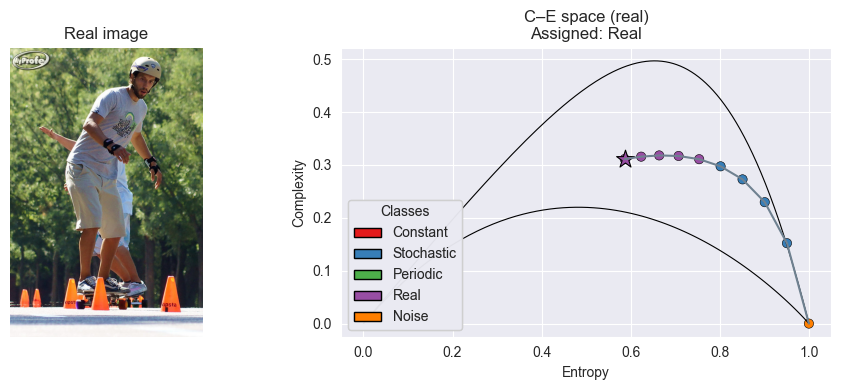
\includegraphics[width=15cm]{real_pair.png}
\caption{%
\textbf{Left:} sample real photograph.
\textbf{Right:} its complexity–entropy trajectory coloured by the
cluster labels learnt in Phase I.
}
\label{fig:pair_real}
\end{figure}

% ------------------  Bad-diffusion example  ------------------
\begin{figure}[htbp]
\centering
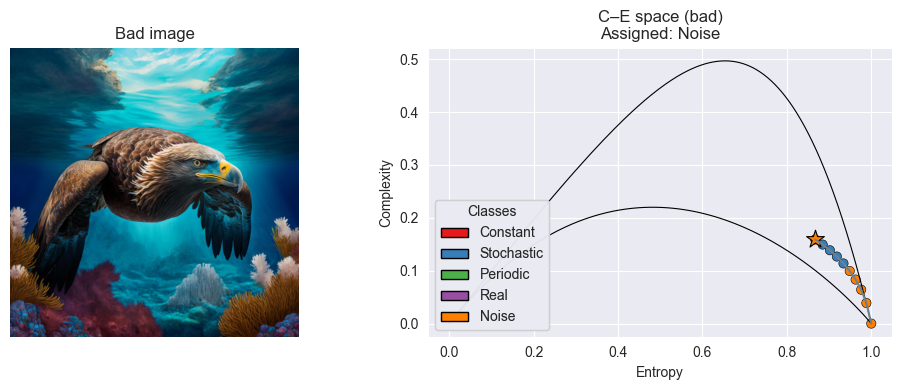
\includegraphics[width=15cm]{bad_pair.png}
\caption{%
\textbf{Left:} hallucinated diffusion output.
\textbf{Right:} the corresponding CE scatter; the point density inside
the \emph{Noise} cluster triggers a positive hallucination flag.}
\label{fig:pair_bad}
\end{figure}

\subsection{Discussion}
The tuned CE+convolution detector not only separates hallucinated
images from \emph{good} generations but — if to assign images from the "Real" cluster as real~\ref{fig:pair_real}, well-generated as "Stochastic"~\ref{fig:pair_good} and generated with hallucination as "Noise"~\ref{fig:pair_bad} — also
acts as an implicit \emph{synthetic-image detector}.  The dual
capability is a by-product of the model’s density estimates in CE
space and does not require any additional supervision.

% ------------------  Good example  ------------------
\begin{figure}[htbp]
\centering
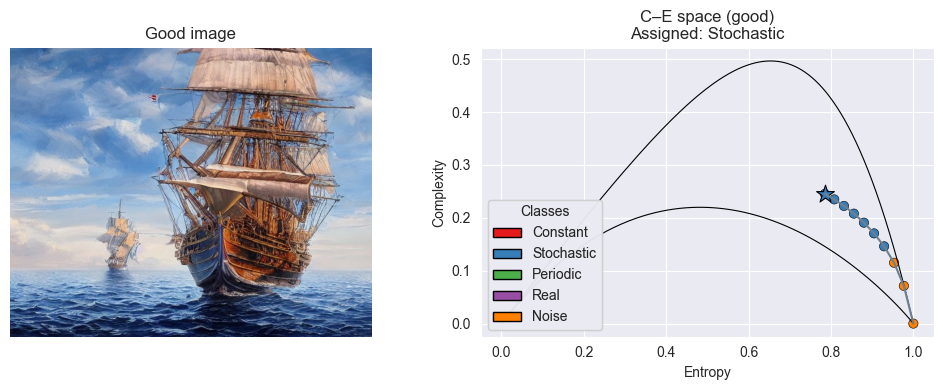
\includegraphics[width=15cm]{good_pair.png}
\caption{%
\textbf{Left:} well-generated image.
\textbf{Right:} classifier output is evident of \textit{stochastic} nature of an image, but without generation errors.
}
\label{fig:pair_good}
\end{figure}

% ------------------ Future Directions  ------------------
\section{Future Directions}

\begin{itemize}
\item \textbf{Adaptive CE parameter tuning.}  
      The current pipeline freezes the embedding order ($d=5$) and delay
      ($\tau=1$), yet \S\ref{sec:grid} shows that silhouette quality is
      sensitive to these hyper-parameters.  Future work should learn
      $(d,\tau)$ automatically — e.g.\ via minimum description length or
      cross-validated stability, and elaborate on larger windows, — so that the CE map self-adapts to each modality.

\item \textbf{Probability-calibrated scoring.}  
      Hallucination decisions are now made by a fixed $p_{\mathrm{hall}}$
      threshold.  Replacing this with another tunable metrics or a calibrated likelihood — learned through temperature scaling or isotonic regression on a held-out
      set — would remove an ad-hoc parameter and enable risk-aware
      downstream use.

\item \textbf{Robustness to perturbations.}  
      Compression, re-sampling and adversarial noise can move CE points
      across cluster boundaries.  A dedicated stress-test suite (JPEG,
      WebP, Gaussian, PGD attacks) is needed to quantify and harden
      detector stability.

\item \textbf{Latent-trajectory scoring.}  
      Embed reverse-diffusion latents into CE space \emph{during}
      sampling; abort or re-sample when a trajectory enters the
      hallucination manifold, turning the detector into a real-time
      safety valve.

\item \textbf{Expanded benchmark and open dataset.}  
      Increase corpus size and domain diversity (text, video, 3-D, medical
      imaging) while publishing images and CE features under a permissive
      licence to foster reproducibility and fair comparison.
\end{itemize}


% ------------------------------------------------------------------
\section{Conclusion}\label{sec:conclusions}

Diffusion models continue to astonish with photorealistic imagery, yet
their tendency to hallucinate artefacts, objects, or entire scenes
poses an unresolved safety risk.  
This thesis framed hallucination detection as a distributional
outlier-problem, mapped raw signals into a two-dimensional
complexity–entropy plane and showed — through a systematic
parameter-sweep — that \textbf{KMeans with \(k=5\)} offers the most stable
and interpretable partition of that space.  
On a canonical time-series benchmark KMeans delivered a silhouette score
of \(0.72\), outperforming both Ward agglomeration and DBSCAN, and it
generalised without modification to image data once a shallow,
tunable convolutional front-end had been added.  
The resulting CE + KMeans pipeline simultaneously (i) flags
hallucinations with high precision, (ii) distinguishes real from
synthetic images as a useful side-effect, and (iii) remains lightweight
enough for real-time screening.  
Taken together, these findings demonstrate that low-dimensional
complexity descriptors, paired with a carefully chosen but simple
clusterer, can form the core of a practical and lightweight hallucination-evaluation
toolkit for current and next-generation diffusion models.

\clearpage
\bibliographystyle{unsrtnat}
\addcontentsline{toc}{section}{References}
\bibliography{references}

\clearpage
\appendix
\section{Additional Experimental Results}
\label{app:experiments}

\begin{table}[htbp]
  \centering
  \small
  \caption{Convolutional layer configurations and their performance metrics.}
  \label{tab:appendix_experiments}
  \begin{tabular}{ccccccc}
    \toprule
    Kernel & Stride & Padding & \#Out & Score & Bad Mean & Non-bad Mean \\
    \midrule
     5 & 1 & 0 & 2 &  0.0046 & 0.9000 & 0.8954 \\
     5 & 2 & 0 & 1 & -0.0011 & 0.9943 & 0.9954 \\
     5 & 2 & 1 & 4 & -0.0013 & 0.9971 & 0.9985 \\
     5 & 1 & 1 & 2 & -0.0022 & 0.9086 & 0.9108 \\
     3 & 2 & 1 & 2 & -0.0057 & 0.9943 & 1.0000 \\
     3 & 1 & 0 & 2 & -0.0059 & 0.8771 & 0.8831 \\
     5 & 1 & 1 & 1 & -0.0073 & 0.8943 & 0.9015 \\
     3 & 2 & 0 & 2 & -0.0079 & 0.9829 & 0.9908 \\
     5 & 2 & 0 & 2 & -0.0095 & 0.9829 & 0.9923 \\
     5 & 2 & 0 & 4 & -0.0099 & 0.9886 & 0.9985 \\
     3 & 2 & 0 & 4 & -0.0125 & 0.9829 & 0.9954 \\
     3 & 1 & 1 & 4 & -0.0130 & 0.8886 & 0.9015 \\
     3 & 1 & 0 & 4 & -0.0136 & 0.8771 & 0.8908 \\
     3 & 2 & 1 & 1 & -0.0152 & 0.9771 & 0.9923 \\
     5 & 1 & 0 & 4 & -0.0158 & 0.9057 & 0.9215 \\
     5 & 1 & 1 & 4 & -0.0165 & 0.8943 & 0.9108 \\
     3 & 2 & 0 & 1 & -0.0169 & 0.9800 & 0.9969 \\
     3 & 2 & 1 & 4 & -0.0169 & 0.9800 & 0.9969 \\
     5 & 2 & 1 & 1 & -0.0169 & 0.9800 & 0.9969 \\
     3 & 1 & 1 & 1 & -0.0187 & 0.8629 & 0.8815 \\
     5 & 2 & 1 & 2 & -0.0198 & 0.9771 & 0.9969 \\
     5 & 1 & 0 & 1 & -0.0255 & 0.8514 & 0.8769 \\
     3 & 1 & 1 & 2 & -0.0382 & 0.8571 & 0.8954 \\
     3 & 1 & 0 & 1 & -0.0510 & 0.8429 & 0.8938 \\
    \bottomrule
  \end{tabular}
\end{table}


\end{document}
